
\documentclass{article}
\usepackage[titletoc, title, toc]{appendix}
\usepackage{hyperref}
\usepackage{graphicx}

\begin{document}
\title{System Design Document for NeedForSpeed (SDD)}
\author{}
\date{}
\maketitle

\tableofcontents

\noindent
\\
\\
\textbf{Version}: 1.0 \\
\textbf{Date}: \today \\
\textbf{Authors}: Anton \\
This version overrides all previous versions.

\section{Introduction}
\subsection{Desgin goals}
The design must be modular to have to possibility to switch GUI.

\subsection{Definitions, acronyms and abbreviations}
\begin{itemize}
  \item GUI, Graphical User Interface
  \item Java, platform independent programming language.
  \item MVC, a way to partition an application with a GUI into distinct parts avoiding
  mixing GUI-code and application code.
  \item JSON, fileformat used for transmitting data in a structured way.
  \item Android, mobile operating system. 
  \item libGDX, framework for developing games in Java.
  \item asset, binary file that contains e.g. sound, texture or font data.
  \item preferences, interface used to write persistent data.
\end{itemize}

\section{System Design}
\subsection{Overview}
The application uses a modified version of the MVC pattern for Android.

\subsubsection{Model Functionality}
The entry point to the model is the World class. We split the model into diffrent classes such as Player, Enemy etc, to keep a modular design.

\subsubsection{Global lookups}
The state of the game is tracked with a global variable. The game state can take on the values paused or running, and is used to decide if we want to render or not in the gamescreen class.

There is a special state called godmode which is mainly used for testing purposes, it basically makes the player invincible.
	
\subsubsection{Event handling}
Generally when the application gets an input from the user it is handled by the controller package which then updates the model accordingly. The view is continuously rendered so a callback from the model is not needed.

Event not handled this way is buttons in menus and the back-key, they are handled directly in the corresponding Screen class. The motivation for this design choice is that these input have nothing to do with the model.

\subsection{Software decomposition}
\subsubsection{General}
INSERT PACKAGE DIAGRAM etc.. \\
The application is decomposed into two main packages, android and core, this is required by libGDX. The android package is for android specific code and assets. The application code resides in the core package.

The core package is futher decomposed into:
\begin{itemize}
  \item view, the GUI part of the game screen, more specific the rendering.
  \item screen, the GUI part of the application.
  \item controller, the controller classes for MVC.
  \item parallax, for parallax background.
  \item highscore, highscore module for reading / writing highscore from file.
  \item gamestate, keeps track of the game state.
  \item model, game logic for the application, model part of MVC.
\end{itemize}

The rendering of the game is decoupled from the GameScreen class to make it easier to debug, modify and add code.

There is also a package for testing.

\subsubsection{Decomposition into subsystem}
The only subsystem present are parallax and highscore.

\subsubsection{Layering}
see figure \ref{fig:stan}

\subsubsection{Dependency analysis}
see figure \ref{fig:stan}


\begin{figure}[h]
  \centering
  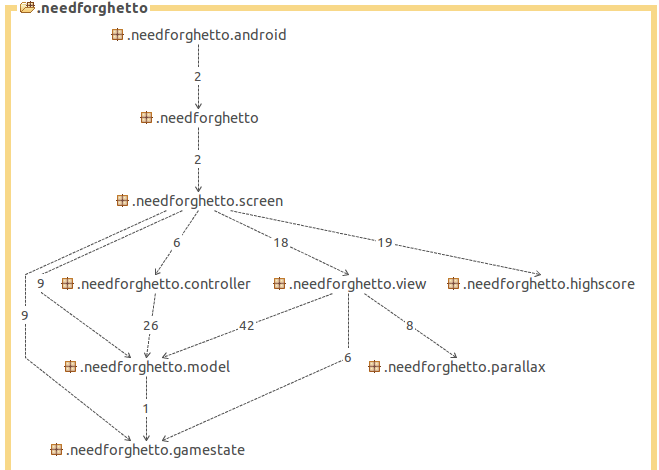
\includegraphics[width=0.8\textwidth]{stan.png}
  \caption{Layering and Dependency analysis}
  \label{fig:stan}
\end{figure}

\subsection{Concurrency issues}
All concurrency is abstracted by libGDX.

\subsection{Persistent data management}
Assets, such as textures, fonts and level information, are persistent and operated on with functions provided by libGDX. Highscore data is handled through the preferences interface. 

Level design data is stored as JSON files.

\subsection{Access control and security}
NA


\subsection{Boundary conditions}
The application is launched and exited as a normal android application.

\section{References}
\begin{enumerate}
  \item ref1
  \item ref2
  \item ...
\end{enumerate}

\newpage
\begin{appendices}
  \section{Class diagrams}
  \section{Other stuff}
\end{appendices}

\end{document}